% Compilar com: latexmk -lualatex I1-covariance__global.tex
% Tabelas e números em tab/ são gerados por ../../info_covariance_assumed_tex.py a partir do manifesto de
% info_covariance_assumed.py. Não editar números à mão: regenerar (DESIGN_SYSTEM 2.08).
\documentclass[11pt,a4paper]{article}
\usepackage[margin=2cm]{geometry}
\usepackage{fontspec}
\usepackage{unicode-math}
\setmainfont{Latin Modern Roman}
\setmathfont{Latin Modern Math}
\usepackage[brazil]{babel}
\usepackage{booktabs,tabularx,array,graphicx,float,longtable}
\usepackage{enumitem}
\usepackage{xurl}
\usepackage[colorlinks=true,linkcolor=blue!50!black,urlcolor=blue!50!black,citecolor=blue!50!black]{hyperref}
\usepackage{xcolor}
\setlength{\parindent}{0pt}
\setlength{\parskip}{0.5em}
\newcolumntype{Y}{>{\raggedright\arraybackslash}X}
\newcommand{\arq}[1]{\texttt{\nolinkurl{#1}}}
\newcommand{\caixa}[2]{\par\noindent\colorbox{#1}{\parbox{\dimexpr\linewidth-2\fboxsep}{#2}}\par}
% generated by info_covariance_assumed_tex.py from I1-covariance__global__cs-rbf.json; do not edit
\newcommand{\valNbins}{917}
\newcommand{\valNobs}{40}
\newcommand{\valNau}{791}
\newcommand{\valNda}{126}
\newcommand{\valCsAuMean}{1{,}000}
\newcommand{\valCsAuHalf}{100{,}0}
\newcommand{\valCsAuZero}{0{,}0}
\newcommand{\valCsAuRank}{1}
\newcommand{\valCsAuEig}{100{,}0}
\newcommand{\valCsDaMean}{1{,}000}
\newcommand{\valCsDaHalf}{100{,}0}
\newcommand{\valCsDaZero}{0{,}0}
\newcommand{\valCsDaRank}{1}
\newcommand{\valCsDaEig}{100{,}0}
\newcommand{\valRho}{1}
\newcommand{\valStepsCs}{200 $\times$ 50\,000}
\newcommand{\valRbfAuMean}{0{,}047}
\newcommand{\valRbfAuHalf}{3{,}4}
\newcommand{\valRbfAuZero}{25{,}7}
\newcommand{\valRbfAuRank}{420}
\newcommand{\valRbfAuEig}{6{,}6}
\newcommand{\valRbfDaMean}{0{,}190}
\newcommand{\valRbfDaHalf}{18{,}4}
\newcommand{\valRbfDaZero}{0{,}2}
\newcommand{\valRbfDaRank}{60}
\newcommand{\valRbfDaEig}{21{,}6}
\newcommand{\valLpt}{0{,}5}
\newcommand{\valLeta}{1}
\newcommand{\valLcent}{10}
\newcommand{\valSigRbf}{c33aba121315}
\newcommand{\valStepsRbf}{200 $\times$ 20\,000}

\makeatletter\newcommand{\tabin}[1]{\@@input #1 }\makeatother  % primitive \input: works inside tables

\title{Covariância experimental suposta: CS global e RBF global\\
\large regra, parâmetros e matriz resultante}
\date{25 de novembro de 2026}
\author{Proposta 1 --- \texttt{1-First\_sensitivity\_test\_global} \quad (I1-covariance, tag \texttt{global})}

\begin{document}
\maketitle
\vspace{-1.5em}

\caixa{blue!6}{\textbf{Resumo.} Na proposta 1, a correlação das incertezas experimentais é \emph{suposta}, não inferida.
Duas regras, ambas com escopo \textbf{global} (todo o sistema de colisão), são aplicadas aos \valNobs{} observáveis da
calibração (\valNbins{} bins: \valNau{} em Au-Au e \valNda{} em d-Au).
\textbf{CS global:} correlação $\rho=\valRho$ entre todos os bins do mesmo sistema. Cada sistema vira um bloco de posto 1,
o caso extremo de um único erro comum a todas as medidas.
\textbf{RBF global:} cada bin é um ponto $(p_T,\eta,\text{centralidade})$, e a correlação é o produto de gaussianas nas
três distâncias, com $L_{p_T}=\valLpt$\,GeV/$c$, $L_\eta=\valLeta$ e $L_{\rm cent}=\valLcent$ p.p. A correlação média
fora da diagonal fica em $\valRbfAuMean$ (Au-Au) e $\valRbfDaMean$ (d-Au): forte só entre bins vizinhos.
Au-Au e d-Au nunca são correlacionados entre si. A diagonal (a variância de cada bin) é a mesma da baseline. Da matriz em
diante, o procedimento é o mesmo de todas as propostas.}

\section{Objetivo}
A verossimilhança da calibração (Mankolli \emph{et al.}, PRC 114, 014905) é
$-2\ln L=(y-\mu(\theta))^{\!\top}(\Sigma_{\rm exp}+\Sigma_{\rm emu})^{-1}(y-\mu(\theta))$. Na baseline,
$\Sigma_{\rm exp}={\rm diag}(\sigma_i^2)$. Este documento registra \textbf{a regra que gera a parte fora da diagonal} em
cada modelo da proposta 1, com todos os parâmetros, e mostra a matriz resultante em números.

\section{Dados: os observáveis da calibração}
A matriz cobre os \valNobs{} observáveis da calibração do 3dglauber, na ordem da verossimilhança
(\arq{mcmc/02_08_sector_input_correlations/bin_index.csv}). Cada bin tem a incerteza da calibração do JETSCAPE no espaço
da verossimilhança: multiplicidades ($dN/d\eta$) entram em log, então
\begin{equation}
\sigma_i=\sqrt{\ln\!\big(1+(\sigma^{\rm exp}_i/y_i)^2\big)}\ \ (dN/d\eta),\qquad \sigma_i=\sigma^{\rm exp}_i\ \ (\text{demais}),
\end{equation}
(\arq{experimental_sector_covariance.likelihood_std}). Os valores bin a bin estão no Apêndice~\ref{ap:sigma}. Para todo
modelo, $\Sigma_{ij}=\sigma_i\sigma_j R_{ij}$ com $R_{ii}=1$: \textbf{só a correlação $R$ muda}.

\section{Método: as duas regras}
\subsection{CS global (compound symmetry, escopo \texttt{system})}
\begin{equation}
R^{\rm CS}_{ij}=\begin{cases}1 & i=j\\ \rho & i\neq j,\ \text{mesmo sistema}\\ 0 & \text{sistemas diferentes}\end{cases}\qquad \rho=\valRho .
\end{equation}
Com $\rho=1$, cada bloco é $\sigma\sigma^{\!\top}$, uma matriz de posto 1 (positiva semidefinida). Fisicamente, é um único
erro comum, com o mesmo sinal, multiplicando todas as medidas do sistema.
Código: \arq{experimental_cs_covariance.compound_symmetry_covariance} (\texttt{groups} = sistema).

\subsection{RBF global em coordenadas físicas comuns}
Cada bin $i$ recebe um ponto $x_i=(p_{T,i},\eta_i,c_i)$:
\begin{itemize}[nosep]
\item \textbf{eixo diferencial} do observável: centro do bin;
\item \textbf{centralidade}: centro da classe da chave do observável (\texttt{cen\_AA\_BB}), ou o centro do bin para
observáveis diferenciais em centralidade;
\item \textbf{eixo integrado} ($\eta$ ou $p_T$): ponto médio da janela de aceitação da medida (Tab.~\ref{tab:coord}).
\end{itemize}
A correlação é
\begin{equation}
R^{\rm RBF}_{ij}=\exp\!\Big[-\Big(\frac{p_{T,i}-p_{T,j}}{L_{p_T}}\Big)^2\Big]\,
\exp\!\Big[-\Big(\frac{\eta_i-\eta_j}{L_{\eta}}\Big)^2\Big]\,
\exp\!\Big[-\Big(\frac{c_i-c_j}{L_{\rm cent}}\Big)^2\Big]\quad(\text{mesmo sistema}),
\end{equation}
com $L_{p_T}=\valLpt$\,GeV/$c$, $L_\eta=\valLeta$ e $L_{\rm cent}=\valLcent$ p.p., os mesmos do RBF sector. Cada razão é
adimensional, então grandezas de unidades diferentes nunca se somam. O fator entre tipos de observável é neutro (1), e
sistemas diferentes têm $R=0$. O produto de gaussianas em coordenadas fixas é positivo semidefinido.
Código: \arq{experimental_global_covariance.global_rbf_covariance}; janelas: \arq{global_rbf_acceptance.json}.

{\scriptsize
\begin{longtable}{@{}r l l l l l l l@{}}
\caption{Coordenadas de cada observável no espaço comum. ``bin'' = eixo diferencial (centro do bin). Última coluna:
janela de aceitação cujo ponto médio dá a coordenada do eixo integrado.}\label{tab:coord}\\
\toprule
\# & sist. & observável & exp. & $p_T$ [GeV/$c$] & $\eta$ & centr. [\%] & janela usada \\
\midrule\endhead
\tabin{tab/coordenadas.tex}
\bottomrule
\end{longtable}}

{\footnotesize
\begin{longtable}{@{}>{\raggedright\arraybackslash}p{6.2cm} >{\raggedright\arraybackslash}p{8.2cm} r@{}}
\caption{De onde vem cada janela (\arq{global_rbf_acceptance.json}, montado a partir dos textos completos).}\\
\toprule
referência & regra da janela & obs. \\
\midrule\endhead
\tabin{tab/referencias.tex}
\bottomrule
\end{longtable}}

\section{Resultados: a matriz}
\subsection{Estrutura por sistema}
\begin{center}\small
\begin{tabular}{@{}l l r r r r r r@{}}
\toprule
modelo & sistema & bins & $\langle R_{ij}\rangle_{i\ne j}$ & pares $R>0{,}5$ (\%) & pares $R=0$ (\%) & posto & 1º autovalor (\%) \\
\midrule
\tabin{tab/sistemas.tex}
\bottomrule
\end{tabular}
\end{center}
O posto e o primeiro autovalor são os da matriz de correlação (o autovalor como fração do traço). No CS global, um único
modo carrega 100\% da variância de cada sistema. No RBF global, Au-Au tem posto \valRbfAuRank{} e nenhum modo passa de
$\valRbfAuEig\%$: a correlação é local.

\subsection{Por observável}
Valores do RBF global. No CS global, toda a coluna seria 1: dentro do observável, com os vizinhos e com os outros observáveis.

{\scriptsize\setlength{\tabcolsep}{3pt}
\begin{longtable}{@{}r l l l r l l l r r r@{}}
\toprule
\# & sist. & observável & exp. & bins & eixo & faixa & $\sigma_i$ & $R$ vizinhos & $\langle R\rangle$ dentro & $\langle R\rangle$ com outros \\
\midrule\endhead
\tabin{tab/observaveis.tex}
\bottomrule
\end{longtable}}
\textit{$R$ vizinhos}: média de $R$ entre bins adjacentes; com espaçamento $\Delta$, $R=e^{-(\Delta/L)^2}$. Por exemplo, $\Delta\eta=0{,}2$
dá $0{,}96$ e $\Delta c=10$ p.p.\ dá $0{,}37$. \textit{$\langle R\rangle$ dentro}: média sobre todos os pares do observável.
\textit{$\langle R\rangle$ com outros}: média com os bins dos demais observáveis do mesmo sistema.

\subsection{Pares de observáveis mais correlacionados (RBF global)}
\begin{center}\small
\begin{tabular}{@{}l l l r@{}}
\toprule
sistema & observável A & observável B & $\langle R_{ij}\rangle$ \\
\midrule
\tabin{tab/pares.tex}
\bottomrule
\end{tabular}
\end{center}
São pares que ocupam o mesmo lugar do espaço comum: mesma centralidade e mesmo $p_T$, medidos por experimentos diferentes.
O RBF global os correlaciona sem saber que são detectores independentes (Sec.~\ref{sec:lim}).

\begin{figure}[H]
\centering
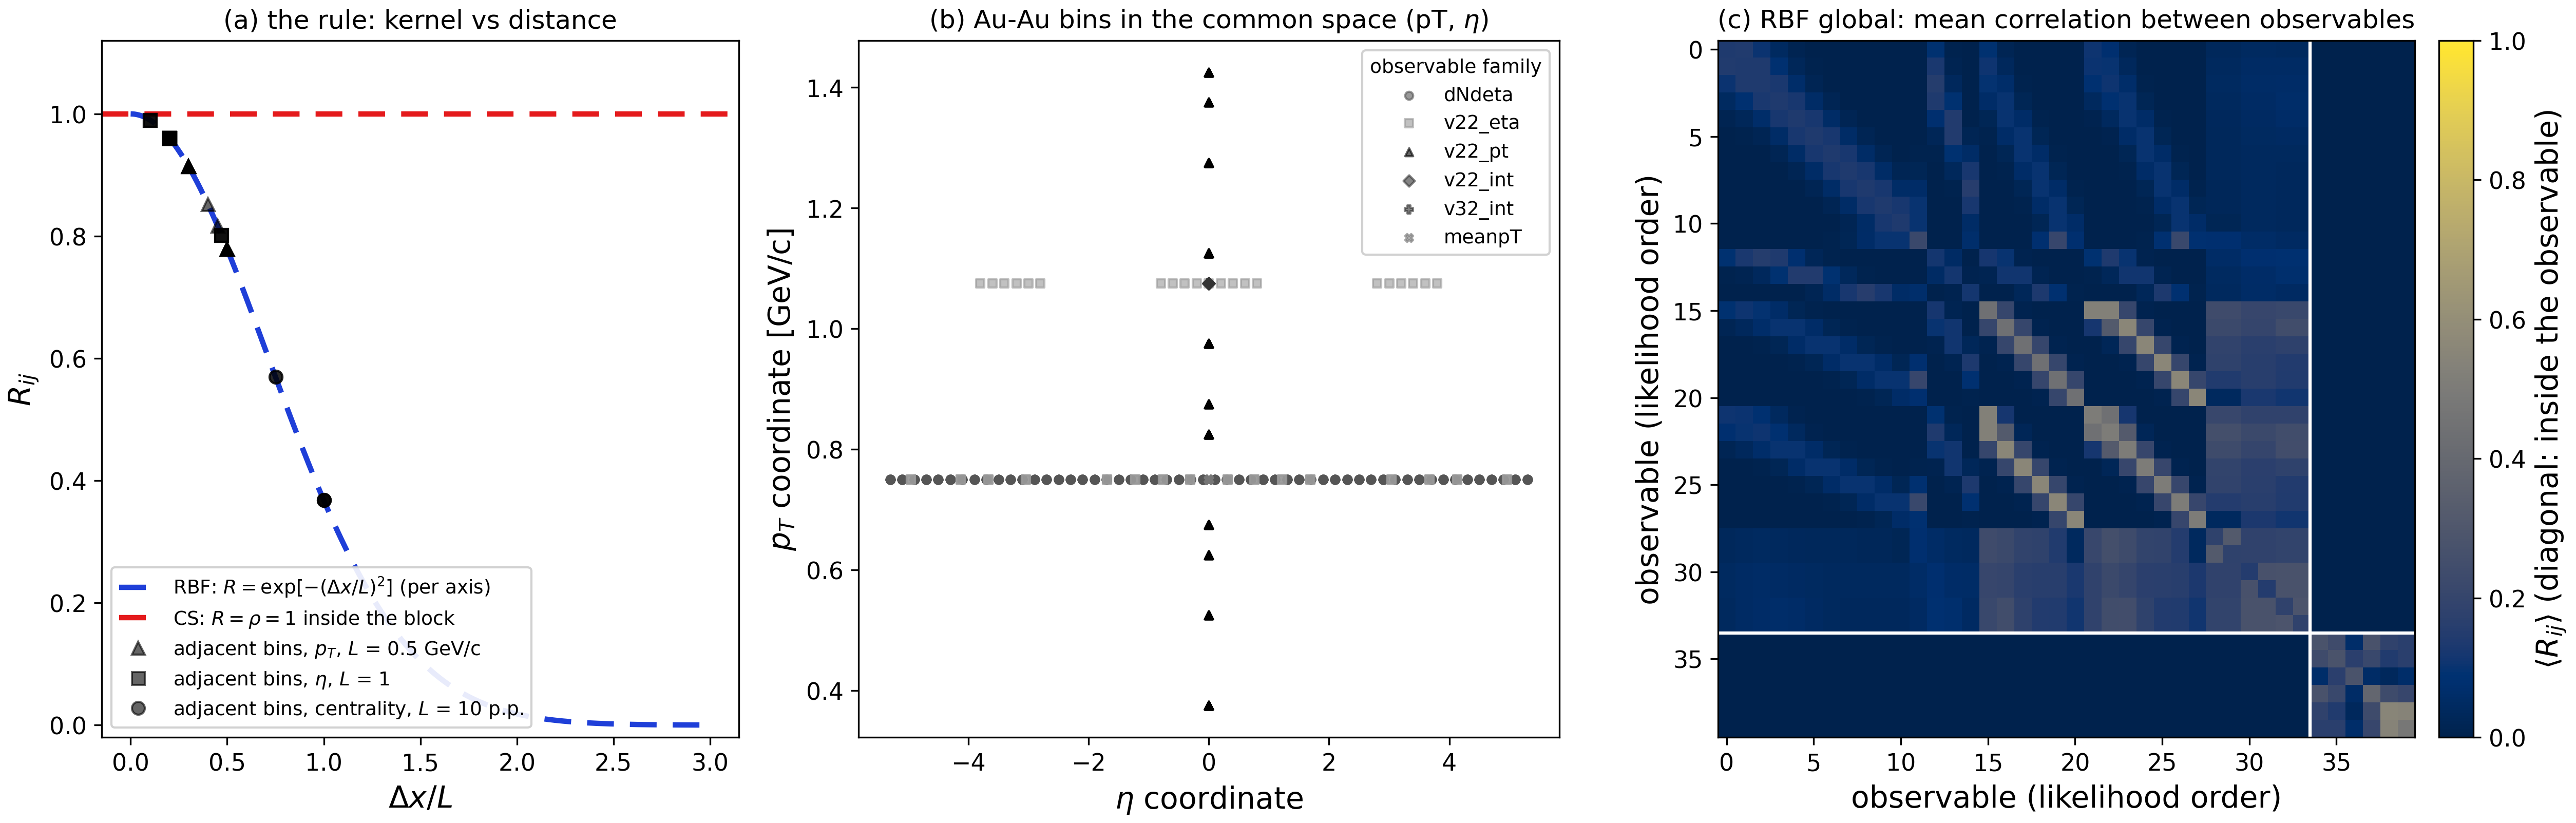
\includegraphics[width=\linewidth]{fig/I1-covariance__global__cs-rbf.png}
\caption{(a) A regra: $R$ contra $\Delta x/L$ (a mesma curva nos três eixos), com o espaçamento entre bins adjacentes de
cada observável; no CS, $R=1$. (b) Bins de Au-Au no espaço comum $(p_T,\eta)$: $dN/d\eta$ e $v_2(\eta)$ ficam no
$p_T$ do ponto médio da janela, e $v_2(p_T)$ fica em $\eta=0$. (c) RBF global: $\langle R\rangle$ entre observáveis (os
40 da calibração; Au-Au à esquerda e acima da linha branca).}
\end{figure}
\begin{figure}[H]
\centering
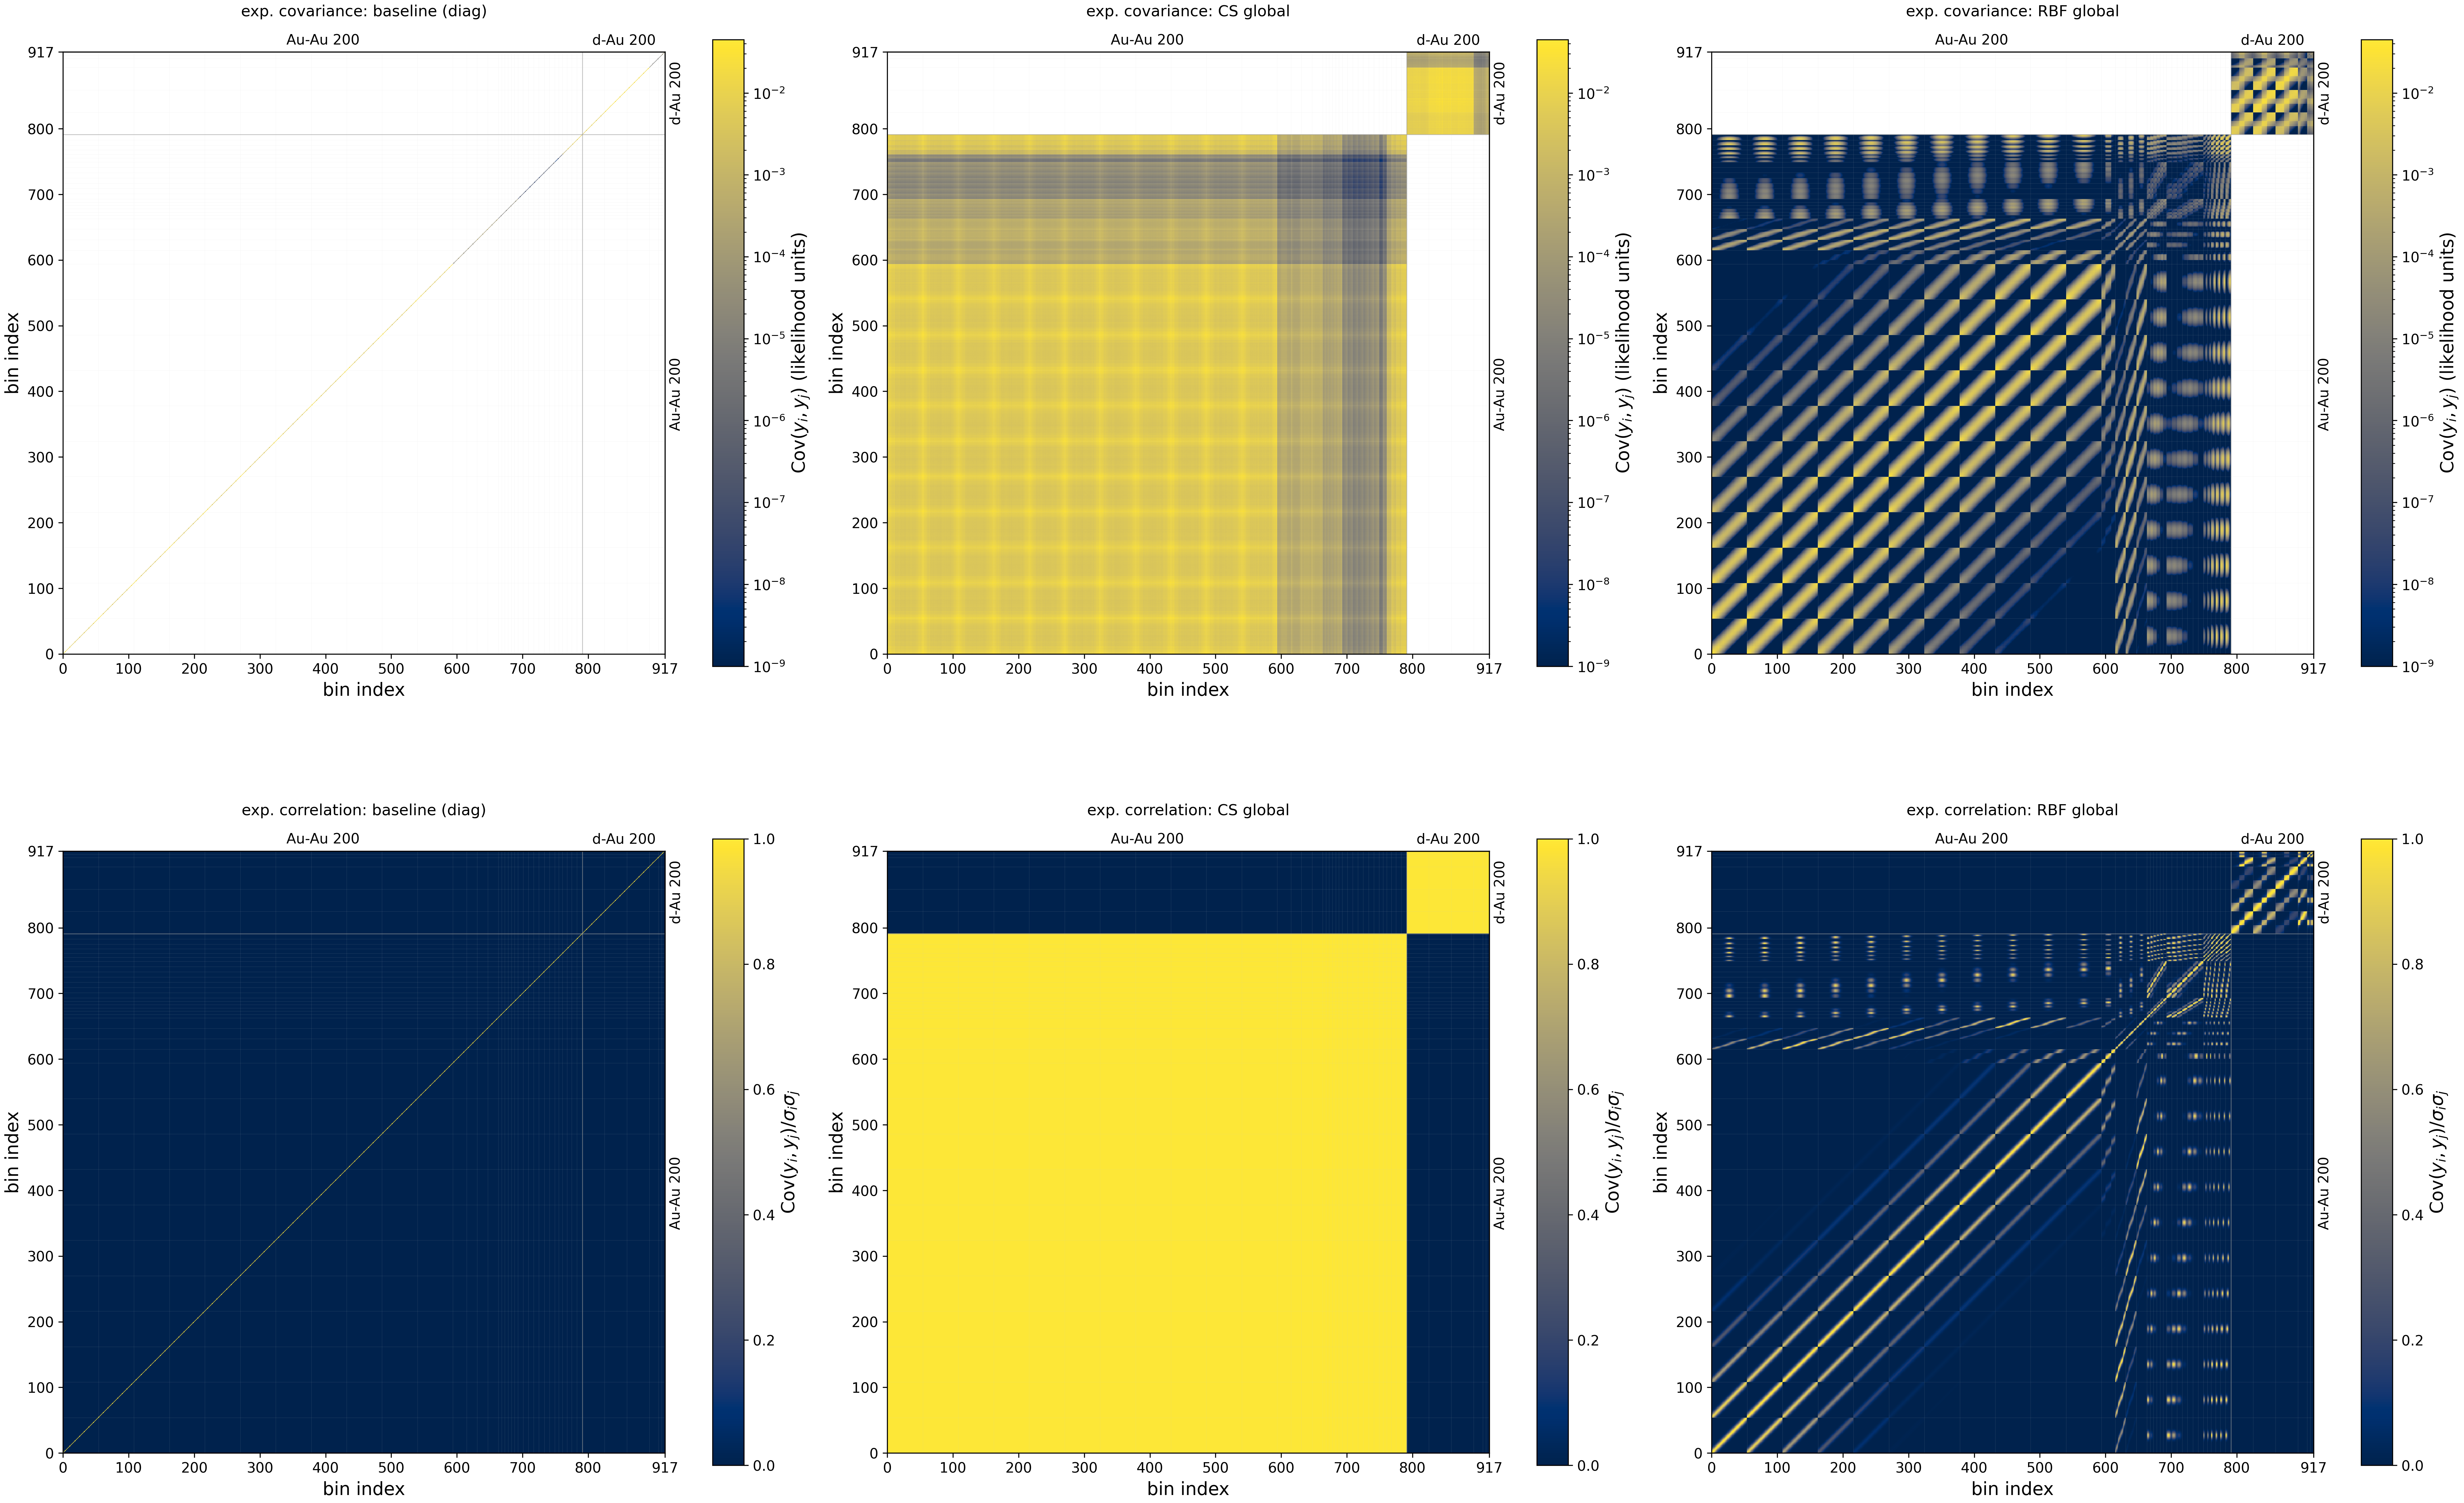
\includegraphics[width=\linewidth]{fig/S2-expcov__global__baseline-cs-rbf.png}
\caption{Covariância (em cima) e correlação (embaixo) nos 917 bins: baseline, CS global e RBF global (\texttt{07\_S2-expcov}).}
\end{figure}
A matriz completa ($\valNbins\times\valNbins$, espaço da verossimilhança) de cada modelo está em
\arq{I1-covariance__global__cs-rbf__<cs|rbf>__matrix_cov.csv} e \arq{..._matrix.npz} (\texttt{cov}, \texttt{corr},
\texttt{sigma}, \texttt{labels}). Elas são reconstruídas com o mesmo código e os parâmetros gravados nas cadeias, e a
diagonal confere com $\sigma_i^2$.

\section{O que é suposto}
\begin{center}\small
\begin{tabularx}{\linewidth}{@{}Y l l@{}}
\toprule
ingrediente & origem & valor \\
\midrule
correlação dentro do sistema (CS) & \textbf{escolha} & $\rho=\valRho$ \\
escopo do CS (todo o sistema) & \textbf{escolha} & \texttt{system} \\
forma do kernel (RBF) & \textbf{escolha} (método do orientador, 24/11) & produto de gaussianas \\
comprimentos $L$ & \textbf{escolha}: iguais aos do RBF sector & $\valLpt$\,GeV/$c$; $\valLeta$; $\valLcent$ p.p. \\
coordenada do eixo integrado & \textbf{convenção}: ponto médio da janela; ``todo $p_T$'' $=[0;1{,}5]$ & Tab.~\ref{tab:coord} \\
fator entre tipos de observável & \textbf{escolha}: neutro & 1 \\
Au-Au $\leftrightarrow$ d-Au & \textbf{escolha} & 0 \\
variância de cada bin & \textbf{calibração} (JETSCAPE), mantida & $\sigma_i$ \\
\bottomrule
\end{tabularx}
\end{center}
Nenhum ingrediente vem de dados de correlação. É isso que diferencia a proposta 1 da 3, onde a correlação do PHOBOS
$dN/d\eta$ é inferida de comparações entre detectores.

\section{Uso na calibração}
\begin{itemize}[nosep]
\item CS global: \arq{mcmc/02_01_global_cs/chain-idf-0-cs-system-rho-1.hdf}, \valStepsCs{} passos de produção
(+20\,000 de burn-in). As figuras usam os primeiros 20\,000.
\item RBF global: \arq{mcmc/02_02_global_rbf/chain-idf-0-rbf-global-c33aba121315.hdf}, \valStepsRbf{}
(+20\,000), job Condor 5078; assinatura da covariância \texttt{\valSigRbf}.
\item Figuras: pastas 01--07 desta proposta, no design system comum.
\end{itemize}

\section{Limitações}\label{sec:lim}
\begin{itemize}[nosep]
\item \textbf{CS global é um limite extremo}: posto 1 por sistema. Toda a incerteza vira um único modo comum, inclusive
entre experimentos e observáveis sem nenhuma relação física.
\item \textbf{RBF global não distingue experimentos}: medidas independentes no mesmo ponto do espaço comum (por exemplo,
$v_2(p_T)$ do PHENIX e do STAR na mesma classe) ficam correlacionadas.
\item \textbf{Coordenada do eixo integrado}: ponto médio da janela, não a média ponderada pelo espectro; ``todo $p_T$''
usa a convenção $[0;1{,}5]$\,GeV/$c$.
\item A cadeia do CS global não grava o atributo de assinatura da covariância; a
reconstrução usa o modelo e o escopo gravados.
\end{itemize}

\appendix
\section{Incertezas da calibração bin a bin}\label{ap:sigma}
$\sigma_i$ no espaço da verossimilhança. $dN/d\eta$: em \% (log). Demais: em unidades de $10^{-3}$ (absolutas). Formato:
centro do bin: $\sigma_i$. Com a regra da Sec.~3, estes valores determinam a matriz inteira.
\par\medskip
{\scriptsize\tabin{tab/sigma.tex}}

\end{document}
